\begin{apendicesenv}

% Imprime uma página indicando o início dos apêndices
\partapendices

\chapter{Códigos-fonte do sistema de médida de bagagens}
\label{apend_Códigos fonte do sistema de médida de bagagens}

    Este apêndice fornece os links para os repositórios dos códigos-fonte desenvolvidos durante a pesquisa para criar o protótipo da solução. Como detalhado ao longo do texto, o produto final consiste em duas partes, o software em Matlab e o código em Arduino, sendo eles:

\begin{itemize}
        \item \href{https://github.com/Vitor0534/Get_obj_dimensions_Kinect}{\textbf{Código em Matlab}}: responsável pela interface de usurário, integração com o sensor Kinect e com a esteira de bagagens. Após a coleta da point cloud é executada a função de medida que computa as dimensões e retorna os dados para o usuário. O link para o repositório é o seguinte \url{https://github.com/Vitor0534/Get_obj_dimensions_Kinect};
        
        \item \href{https://github.com/Vitor0534/CodigoPrototipoEsteira}{\textbf{Código em Arduino}}: responsável pela automação do hardware do sistema. Realiza o controle da esteira e contém um módulo de configuração via porta serial. A interface via porta serial reconhece diversos comandos padronizados para alteração de velocidade, direção e precisão do controlador RPM, também é possível fazer o mesmo por um painel físico. O link para o repositório é o seguinte \url{https://github.com/Vitor0534/CodigoPrototipoEsteira};
\end{itemize}

% \begin{minted}{Matlab}
% %Posteriormente serão inseridos códigos aqui

% \end{minted}

\chapter{Interface de usuário}
\label{apend_Interface de usuário}

    O presente apêndice ilustra a interface de usuário desenvolvida para o protótipo, tal interface pode ser observada na Figura \ref{fig:softwareUI}. Esse recurso foi implementado para facilitar a operação do sistema e realização de testes com diferentes parâmetros. 

        \begin{figure}[h!]
           \centering
           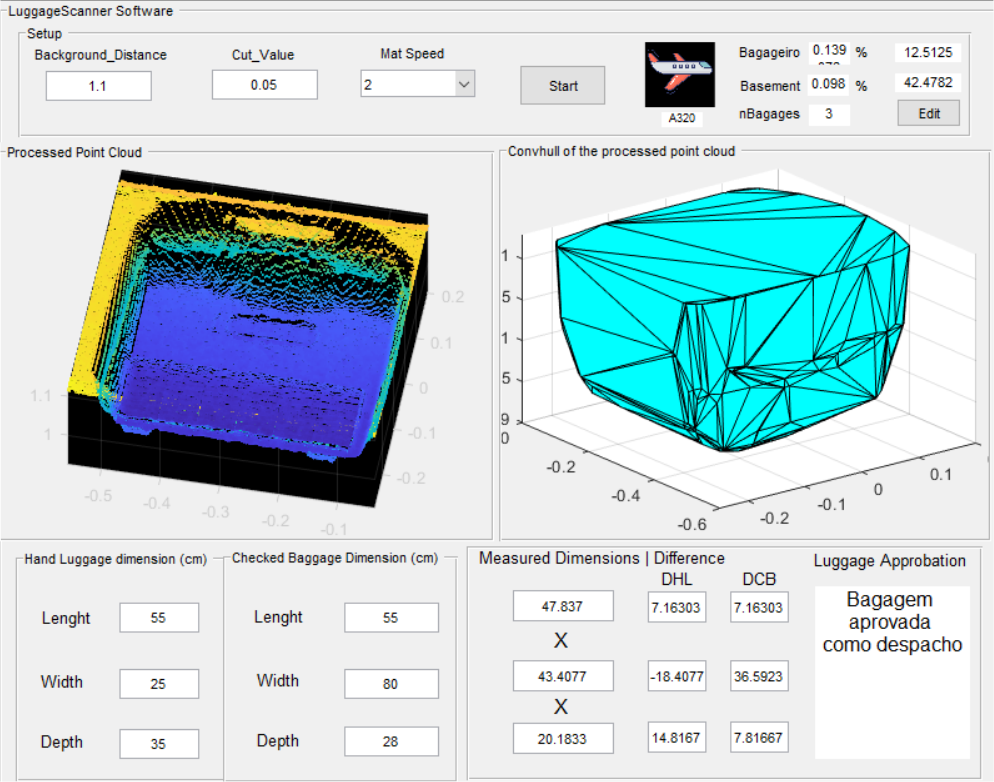
\includegraphics[width=0.8\textwidth]{imagens/softwareUI.png} 
           \caption{Interface de usuário do protótipo desenvolvido na presente pesquisa}
           \label{fig:softwareUI}
        \end{figure}

    Dentre as ações disponibilizadas existe a opção de indicar as dimensões máximas de bagagens de mão e despacho (comprimento, altura e profundidade) e, também, iniciar o processamento. As demais opções podem ser pontuadas na seguinte ordem:

\begin{itemize}
        \item Setup: permite a configuração de parâmetros do sensor, tal como distancia a base, valor de corte e velocidade da esteira. Também contém elementos para visualização do volume em $m^3$ consumido no bagageiro/porão da aeronave e o número de bagagens aprovadas;
        \item Visualização de \textit{point cloud}: a \textit{point cloud} e o polígono mínimo são plotados nos dois gráficos centrais;
        \item Campo de dimensões medidas: componente de saída que irá listar os resultados da medida da bagagem. Os dados são disponibilizados em termos de comprimento, altura e profundidade. O campo "DHL" disponibiliza a diferença entre o valor máximo permitido para bagagem de mão e o obtido na medida, o "DCB" faz o mesmo para bagagem de despacho. O campo de aprovação de bagagem apenas mostra uma mensagem de bagagem aprovada ou não.
\end{itemize}








\end{apendicesenv}